\chapter{Solution Design}
This chapter details and explains various aspects of the solution design. It begins with a explanation of the envisioned implementation of the solution in the clothing industry ecosystem. This is followed by a detailed account of the design process used to create the solution and lastly, an extensive overview of the experimental process used to test the solution.

\section{Implementation Design}

\subsection{Overview}
The solution aims to form part of larger practical implementation that will be applicable and provide relief in all three clothing channels mentioned in Section \ref{clothingIndustryContext}. However, in order to understand the needs the implementation must address, an analysis of pain points of consumers and producers in each channel must be performed. Shown in Table \ref{tab:conProdPainPoints} is a summary of such an analysis.

\begin{table}[htbp]
	\centering
	\caption{Pain points of consumers and producers in each of the three channels}
	\begin{tabularx}{\textwidth}{|Y|Y|Y|}
		\toprule
		& 
		\textit{\textbf{Consumers}} & 
		\textit{\textbf{Producers}} \\
		\midrule
		\textit{\textbf{Retail}} & 
		\begin{itemize}
			\item Visiting stores is time consuming
			\item Trying clothes on is tedious
			\item The correct size is often not available 
		\end{itemize} & 
		\begin{itemize}
			\item Dressing rooms waste valuable space
			\item Trying on clothes pose a security risk and require resources to control
			\item Significant costs are incurred during exchanges 
		\end{itemize} \\
		\midrule
		\textit{\textbf{Online}} & 
		\begin{itemize}
			\item Difficult to choose the correct size
			\item Not sure how the item will look on body
			\item Frustrating to exchange if item is incorrect
		\end{itemize} & 
		\begin{itemize}
			\item Exchanges severely impact their profitability
			\item Experience lower sale volume due as they cannot provide a complete customer experience
		\end{itemize}\\
		\midrule
		\textit{\textbf{Tailoring}} & 
		\begin{itemize}
			\item Only available for specialised clothing
			\item The process is time consuming
			\item There is always delay between getting measured and picking up clothing
		\end{itemize} & 
		\begin{itemize}
			\item Time required to complete measurements limits productivity
			\item Measurements can only take place in person with a trained tailor
		\end{itemize} \\
		\bottomrule
	\end{tabularx}%
	\label{tab:conProdPainPoints}%
\end{table}%


The aim of the overall implementation is to alleviate stresses on both consumers and suppliers that are inherent to the status quo.  In order to achieve this, the implementation will consist of the following key components: 

\begin{itemize}
	\item A compact, expedient and easy to use system that accurately measures the body parameters of a customer and provide clothing suggestions
	\item A platform that retains this customer information and creates a digital profile accessible to the customer and shareable between retailers  
	\item An intuitive interface that allows the customer to seamlessly get advise on clothing at his/her retailers of choice	
\end{itemize} 

These key components were developed into a more detailed end-to-end journey of the implementation. This is given in the following section.

\subsection{End-to-End Implementation Journey}
A diagram illustrating the high-level functioning of the entire implementation is seen in Figure \ref{fig:endToEndImplementation}.

\begin{figure}[ht]
	\centering
	{%
		\setlength{\fboxsep}{0pt}%
		\setlength{\fboxrule}{0.5pt}%
		\fbox{
			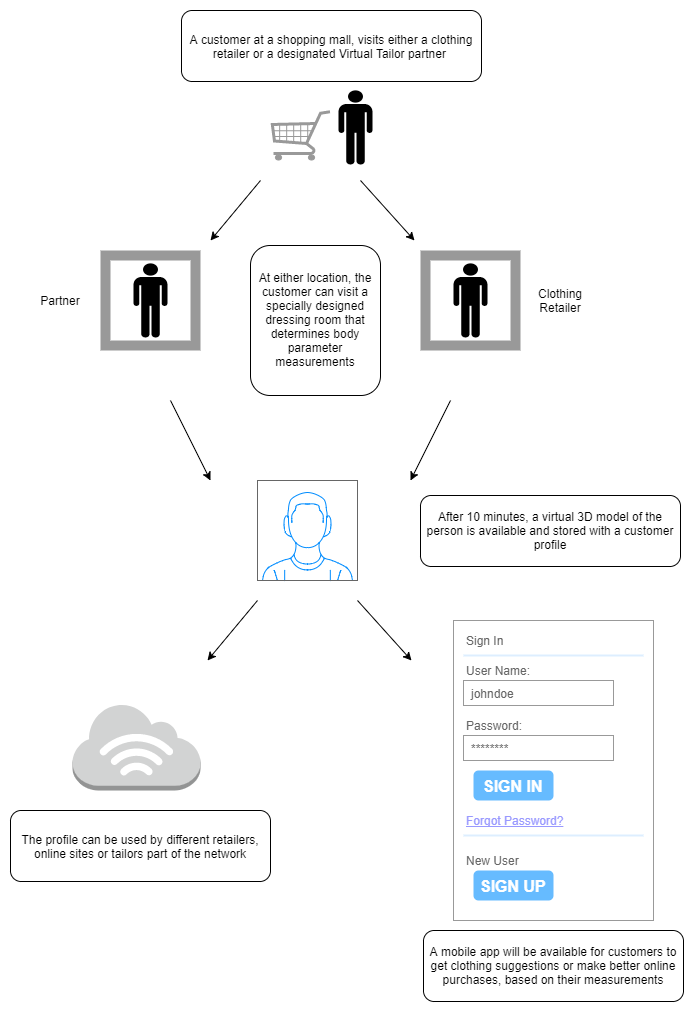
\includegraphics[width=0.7\textwidth]{End_to_End_Implementation.png}
	}}
	\caption{An illustration of the End-to-End journey of the envisioned implementation}
	\label{fig:endToEndImplementation}
\end{figure}

The implementation can be broken down into three major subsystems that are mentioned and explained in the following subsections:

\subsubsection{Measurement System} \label{measureSystem}
This system's main purpose is to be able to determine the personalised body parameters of a customer and then generate a full 3D model of their body to provide useful information such as suggestions for clothing sizes. It will achieve this by using a Kinect, or another device with depth sensing capabilities. 

The vision is that the Kinect would be integrated into a specially designed room. The customer would need to step into this room and hold certain poses. The Kinect, together with a back-end processing unit, would then create a full 3D. The entire process from start to finish should be less than ten minutes. 

This is the most integral part of the implementation as it allows for the realisation of the other two subsystems mentioned below. The main focus of this project is creating a first attempt at this subsystem. As such, its design and functioning are covered in great detail in Section \hl{(Measurement Design)}. 

\subsubsection{Store Integration}
In order to facilitate the measuring process, a room, integrated with a Kinect, would need to be placed at a convenient location for customers. Two possibilities are explored here:

\paragraph{Traditional Retailers}
There is a significant incentive for these retailers to provide a space for this "virtual room". (Expanded upon in Section \hl{(Benefits)}) As such, given that this system aims to limit the need for physically trying on clothes, one of the spaces previously dedicated to a dressing room could be upgraded to this new virtual room. Minimal change to the infrastructure would be required and this also frees up more space as unused dressing rooms can be replaced. 

In this instance, consumers would be able to record their measurements when visiting the clothing store. The measurements would be recorded and they can continue their clothing shopping with a better understanding of sizes. Since the customer would already be shopping and the process only needs to occur once (Assuming no change to the customer's body), it seems likely that their would be buy-in into the system.

\paragraph{Partners}
If there is enough interest by various companies, a measurement booth can be built in a commonly used location (I.e. in a shopping mall). Any customer visiting this booth, would automatically have profiles at all the companies sharing the booth. This is the other alternative if a specific company does not want to dedicate their floor space for this solution, but rather outsource it. This would also be the most likely method in which an online store can partake to allow for digital profiles of their shoppers to be created.

\subsubsection{Cloud Management of Profile}
Once the measurements of a person are determined and a digital profile is created, that information can now be more easily transferred. Partnerships may be made between clothing companies, online companies and even perhaps tailors. They may agree to share this information for an agreed upon amount and allow the costumer to have clothing suggestions for all the stores they shop at. Alternatively, a single online platform may be created that stores all these profiles and if a clothing supplier partners up with it, it can then provide information to the customers regarding the supplier's specific line of clothing.

\subsubsection{Potential Benefits}
The effective and practical implementation of the above system has significant potential benefits for each of the stakeholders. Table \ref{tab:conProdBenefits} contains a summary of the potential benefits for consumers and producers in the different channels.

\begin{table}[htbp]
	\centering
	\caption{Potential benefits for consumers and producers in each of the three channels}
	\begin{tabularx}{\textwidth}{|Y|Y|Y|}
		\toprule
		& 
		\textit{\textbf{Consumers}} & 
		\textit{\textbf{Producers}} \\
		\midrule
		\textit{\textbf{Retail}} & 
		\begin{itemize}
			\item No longer need to waste time and effort trying on clothes
			\item Significantly reduces the shopping time required
			\item Knowing exact sizes allows for calling ahead to check for availability
		\end{itemize} & 
		\begin{itemize}
			\item More floor space to use more productively
			\item Alleviates the security risk of trying on clothes
			\item Will likely cause a reduction in costs due to exchanges
		\end{itemize} \\
		\midrule
		\textit{\textbf{Online}} & 
		\begin{itemize}
			\item Knowing exact sizes reduces uncertainty of online shopping
			\item Potential for clothe viewing using augmented reality
			\item Reduces the need to exchange
		\end{itemize} & 
		\begin{itemize}
			\item Reduces the costs associated with returns
			\item Can expect an uptick in sales
			\item No longer need to have an overly lenient returns policy
		\end{itemize}\\
		\midrule
		\textit{\textbf{Tailoring}} & 
		\begin{itemize}
			\item Process is quick and only needs to happen once
			\item Measurements can be sent ahead of time to reduce delay
			\item No need to visit tailor before collection
		\end{itemize} & 
		\begin{itemize}
			\item Reduce time taken for readings will improve productivity
			\item No longer limited by number of skilled tailors
			\item Might make mass production of custom clothing possible
		\end{itemize} \\
		\bottomrule
	\end{tabularx}%
	\label{tab:conProdBenefits}%
\end{table}%

\section{Component Level Design}
This section details the design process used to create the measurement system mentioned in Section \ref{measureSystem}. It first begins with the selection process used to choose both the hardware and software of the system. It then proceeds into the design of the algorithm, which forms the largest part of the design process.

\subsection{Component Selection}

\subsubsection{Hardware}

\paragraph{Depth Sensor}
When this project was first proposed, no hardware system was specified for use, However, it was indicated that a depth sensor should be the first technology explored to achieve this. Depth sensor technology has extensively been involved in projects performing analysis on human bodies. As such, this suggestion was used and a depth sensor was the hardware device chosen for the project. 

The next step was to determine the particular depth sensor used. Initially, due to ease of availability, sensors such as the Intel RealSense, Asus XtionPRO Live and the Kinect for Xbox 360 were considered. However, it was swiftly decided that the Kinect be the sensor of choice. The reasons for this are given below:

\begin{itemize}
	\item The Kinect has in built skeleton tracking functionality
	\item Microsoft has released an SDK (Software Development Kit) that allows for effective interfacing with the Kinect 
	\item Many previous research papers have utilised the Kinect and thus the support for it is extensive
	\item This project is for research purposes and there are no license conflicts with using the Kinect in this capacity
\end{itemize}

\paragraph{Kinect Choice}
The next significant decision, however, was the version of Kinect used for the project. The first part of the process was the decision between the Kinect for Xbox 360 (Version 1 - v1) or the Kinect for Xbox One (Version 2 -v2). 

The Kinect v2 uses ToF (Time-of-Flight) technology that has been shown to improve its accuracy. It also does not falter as significantly as the Kinect v1 in extreme constitutions such as darkness or direct sunlight. It also has a better working range as the accuracy of the Kinect v1's depth sensor degrades exponentially as the distance away from the sensor increases whereas the Kinect v2 stays almost constant over the same range. \cite{kinectComp2011} This can be seen in Figure \ref{fig:kinectV1V2Depth}. 

\begin{figure}[ht]
	\centering
	{%
		\setlength{\fboxsep}{0pt}%
		\setlength{\fboxrule}{0.5pt}%
		\fbox{
			\includegraphics[width=0.7\textwidth]{kinectV1vsV2Depth.png}
	}}
	\caption{A graph showing the comparison of the accuracy and standard deviation of the Kinect v1 and Kinect v2 as distance from the sensor increases \cite{kinectComp2011}}
	\label{fig:kinectV1V2Depth}
\end{figure}

However, despite these performance advantages of the Kinect v2, the Kinect v1 was chosen for this project for the following reasons:

\begin{itemize}
	\item The Kinect v1 was already available for use and the Kinect v2 was not
	\item The tolerance advantage of the Kinect v2 to extreme condition is mitigated by:
	\begin{itemize}
		\item The Kinect will perform in normal conditions - I.e. It will be indoors, in a well lit room with no direct light shining on the Kinect (Mentioned more in detail in \hl{(Experiment Design Ref)}).
		\item The Kinect v1 and v2 have very similar performance in normal conditions \cite{kinectComp2011}
	\end{itemize}
	\item Skeletal tracking only works effectively up to a distance of 3.5m (Section \hl{(Skel Tracking Ref)}) and the difference in accuracy of the depth sensors only becomes significant after 3m as seen in Figure \ref{fig:kinectV1V2Depth}. Working within the 3m range makes the accuracy difference negligible.
\end{itemize}

Lastly, the Kinect for Xbox 360 was chosen instead of the Kinect for Windows for the following reasons:

\begin{itemize}
	\item The Kinect for Xbox 360 with a USB adapter was already available
	\item These two Kinects are almost functionally identical, except for near range depth mode being unavailable in the Kinect for Xbox \hl{(Kinect Near Range Mode)}
	\item Near Range mode is not utilised in this project and thus, this lack of functionality is no essential.
\end{itemize}

\subsubsection{Software}
The software used to design this solution was largely dictated by the choice of the Kinect as the underlying hardware. 

In order to maximise the functionality of the Kinect, the Kinect for Windows SDK was utilised. This SDK provides an API (Application Programming Interface) for the Kinect in both C\# and C++ programming languages. 

C\# was chosen as the language in which to build the solution as at this stage of the project, finite control over aspects of the Kinect offered by the C++ is not necessary. 

Also provided with the SDK, is Microsoft Toolkit for the Kinect. This toolkit contains further functionality over and above those provided by the SDK. Included with the toolkit are full coded examples of different basic applications using the Kinect SDK and toolkit to demonstrate how to use them. Each of these examples come with their own documentation and are in the form of Visual Studio Projects.

Visual Studios is Microsoft's official IDE (Integrated Development Environment). It supports development in a variety of languages including C\# and C++. Due to the SDK reliance on Visual Studios, its wide functionality and extensive online support, it was chosen as the IDE for this project. 

\hl{(Include NUI Info and Samples used + Documentation)}

\subsection{Algorithm Design}
As mentioned above, the main part of this solutions design was in the design of the algorithms required to make the measurement subsystem a reality. This section details the design process followed and begins with an overview of the created system and how it functions. Proceeding that is an explanation of the system's architecture and finally, extensive details about the functional blocks that form the measurement subsystem. 

\subsubsection{Overview}


\subsubsection{Architecture}


\subsubsection{Functional Blocks}

1) Windows examples used - Background Removal, Colour Stream and Skeleton Tracking - NB - Why BackgroundRemoval instead of own method
3D Points - No calibration

2) Run through of algorithm
- Background Removed frame
- Send image to separate class for processing
- Create array with background removed pixels
- Draw skeleton on image
- Create axes for measurement - Perpendicular or straight depending on particular measurement

\section{Experimental Design}
- Constraints - Men, distance from Kinect, height of Kinect, Number of views, 3D Modelling, control distance - box of 0.5m
- UI to run simulated dressing room
- Volunteer to pose as instructed by person controlling UI
- Take measurement of front
- Take left
- Take back
- Take right 
- At each point, take actual readings with uncertainty
- Note: Did not use correction in \cite{nonContact2017}
- For one volunteer, take 5 readings in relatively the same pose - Determine uncertainty 